\section{Non-linear Wave Equation in 1+1 Dimensions with Periodic Boundary Conditions}
\label{sec:non_linear_wave}

The next step towards our goal is to solve a non-linear Wave Equation, since we need artificial dissipation for both this problem and the Einstein Equations, as they are non-linear.

Similarly to what we did with the linear wave equation, we will be solving the non-linear wave equation in its PDE system form (equation \eqref{eq:non_linear_simple_wave}) with nonlinear coefficient $m=2$ in 1+1 dimensions with the Cauchy boundary conditions in equation \eqref{eq:sin_IC} and periodic boundaries of period $L = 1$. We solved the equation with the same resolutions as we did in section \ref{sec:simple_wave}, so we will keep the nomenclature previously defined. However, even though we solved this equation until $t = 4.5$, the pointwise convergence graphs only show until the time $t = 3.5$, since the error grows very fast after that, making the graphs impossible to analyze.
 

The results for the 2nd-order accuracy in space and 1st-order accuracy in time solution are in figures \ref{fig:norm_non_linear_simple_wave_2nd_order-diss} and \ref{fig:point_non_linear_simple_wave_2nd_order-diss}, where we used Kreiss Oliger dissipation with a dissipation coefficient $\sigma = 0.02$.

The intensity plot showing the solution is represented in figure \ref{fig:intensity_non_linear_simple_wave_2nd_order}.

\begin{figure}[t!]
    \centering
    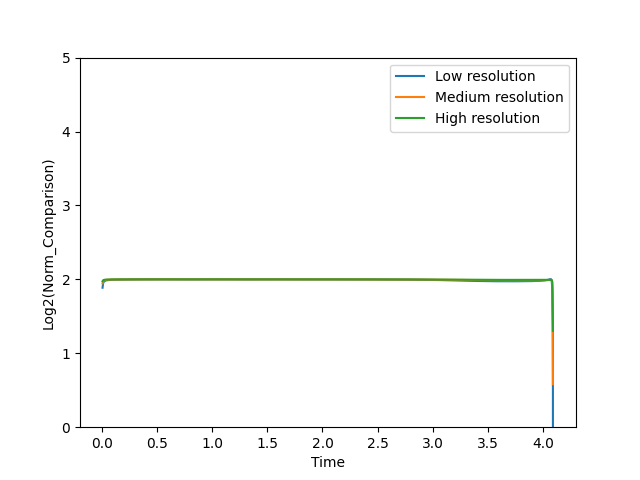
\includegraphics[width=\columnwidth]{Images/non_linear_simple_wave-2nd-norm-diss.png}
    \caption{Norm convergence of the solution to the non-linear wave equation in 1+1 dimensions (with artificial dissipation $\sigma = 0.02$) with periodic boundary conditions and initial conditions represented in equation \eqref{eq:sin_IC} with $m = 2$ in the 2nd-order accurate in space and 1st order accurate in time code}
    \label{fig:norm_non_linear_simple_wave_2nd_order-diss}
\end{figure}

\begin{figure}[t!]
    \centering
    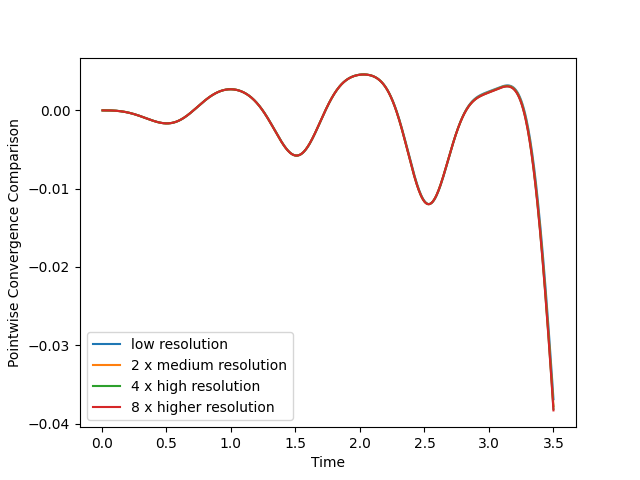
\includegraphics[width=\columnwidth]{Images/non_linear_simple_wave-2nd-point-diss.png}
    \caption{Pointwise convergence for $x = 0$ of the solution to the non-linear wave equation in 1+1 dimensions (with artificial dissipation $\sigma = 0.02$) with periodic boundary conditions and initial conditions represented in equation \eqref{eq:sin_IC} with $m = 2$ in the 2nd-order accurate in space and 1st order accurate in time code}
    \label{fig:point_non_linear_simple_wave_2nd_order-diss}
\end{figure}

\begin{figure}[t!]
    \centering
    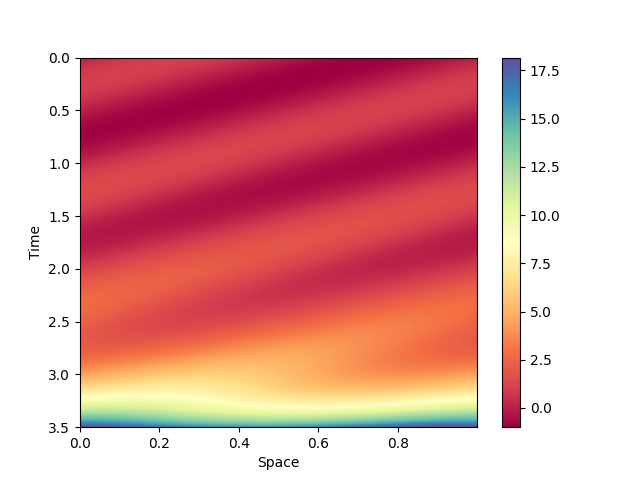
\includegraphics[width=\columnwidth]{Images/non_linear_wave-2nd_order-Intensity.png}
    \caption{Intensity plot of the solution to the non-linear wave equation in 1+1 dimensions (with artificial dissipation $\sigma = 0.02$) with periodic boundary conditions and initial conditions represented in equation \eqref{eq:sin_IC} with $m = 2$ in the 2nd-order accurate in space and 1st order accurate in time code}
    \label{fig:intensity_non_linear_simple_wave_2nd_order}
\end{figure}

From these figures, we can still observe a clean convergence until the solution grows uncontrollably. This is in fact a good sign, as the solutions to this equation analytically diverge. Since we have a clean convergence up until what we can assume is the analytical singularity, we can conclude that our code is working.

We also solved this problem with a 4th-order accuracy in space and 1st-order accuracy in time, where we used a dissipation coefficient $\sigma = 0.007$. These results are found in the appendix.